\documentclass[10pt,norsk,a4paper]{article}
\usepackage[utf8]{inputenc}
\usepackage[T1]{fontenc}
\usepackage[norsk]{babel}
% - PDF-relatert
\usepackage{hyperref,pdfpages,hypcap}
\hypersetup{colorlinks=true,allcolors=.}
\newcommand\fhref[2]{%
	\href{#1}{#2}\footnote{\url{#1}}%
}
% Andre pakker
\usepackage[cm]{fullpage}
\usepackage{parskip,multicol,textcomp,amssymb,graphicx,color}
% - Korte og enkle bruk av listenummerering
\usepackage[shortlabels]{enumitem}
% - Korreksjon av fotnoter i seksjoner/overskrifter
\usepackage[stable]{footmisc}
% - Skrifttype
\usepackage[bitstream-charter]{mathdesign}
% - Kommentarer
\usepackage{comment}


\title{Ekstraordinær generalforsamling \\
	Høsten 2018\\[3cm]
	
\includegraphics[width=0.5\textwidth]{cyb-logo.eps}\\[-.5cm]}
\date{27.\ november 2018}
\author{Cybernetisk Selskab}

% Blank header, samt footer med side x av y
\usepackage{fancyhdr}
\pagestyle{fancy}
\renewcommand{\headrulewidth}{0pt}
\fancyhead{}
\cfoot{Side~\thepage\ av~\pageref*{lastpage}}

%DIF PREAMBLE EXTENSION ADDED BY LATEXDIFF
%DIF UNDERLINE PREAMBLE %DIF PREAMBLE
\RequirePackage[normalem]{ulem} %DIF PREAMBLE
\RequirePackage{color}\definecolor{RED}{rgb}{1,0,0}\definecolor{BLUE}{rgb}{0,0,1} %DIF PREAMBLE
\providecommand{\DIFaddtex}[1]{{\protect\color{blue}\uwave{#1}}} %DIF PREAMBLE
\providecommand{\DIFdeltex}[1]{{\protect\color{red}\sout{#1}}}                      %DIF PREAMBLE
%DIF SAFE PREAMBLE %DIF PREAMBLE
\providecommand{\DIFaddbegin}{} %DIF PREAMBLE
\providecommand{\DIFaddend}{} %DIF PREAMBLE
\providecommand{\DIFdelbegin}{} %DIF PREAMBLE
\providecommand{\DIFdelend}{} %DIF PREAMBLE
%DIF FLOATSAFE PREAMBLE %DIF PREAMBLE
\providecommand{\DIFaddFL}[1]{\DIFadd{#1}} %DIF PREAMBLE
\providecommand{\DIFdelFL}[1]{\DIFdel{#1}} %DIF PREAMBLE
\providecommand{\DIFaddbeginFL}{} %DIF PREAMBLE
\providecommand{\DIFaddendFL}{} %DIF PREAMBLE
\providecommand{\DIFdelbeginFL}{} %DIF PREAMBLE
\providecommand{\DIFdelendFL}{} %DIF PREAMBLE
%DIF HYPERREF PREAMBLE %DIF PREAMBLE
\providecommand{\DIFadd}[1]{\texorpdfstring{\DIFaddtex{#1}}{#1}} %DIF PREAMBLE
\providecommand{\DIFdel}[1]{\texorpdfstring{\DIFdeltex{#1}}{}} %DIF PREAMBLE
%DIF END PREAMBLE EXTENSION ADDED BY LATEXDIFF

\begin{document}

\maketitle{}
\newpage
\tableofcontents

\part*{Agenda}

\section{Valg av møteleder}

\section{Valg av referent}

\section{Valg av protokollunderskrivere}

\section{Valg av tellekorps}

\section{Godkjenning av innkalling}

\section{Godkjenning av dagsorden}

%\newpage



\section{Valg av promoteringssjef til hovedstyret}
Man velges inn i hovedstyret for ett år av gangen.

Hovedstyret ønsker å informere om at eventuelle kandidater kan stille på ekstraordinær generalforsamling, spesielt ettersom etterfylling kun er gyldig frem til neste generalforsamling.


\section{Vedtektsendringer}

Hovedstyret har enstemmig vedtatt å anbefale generalforsamlingen at samtlige forslag aktivt stemmes for.

Måter å håndtere stemmingen:

\begin{enumerate}
	\item Stemme for ett og ett forslag.
	\item Hovedstyret anbefaler videre at forslag 8.1 stemmes for alene, da det ikke er avhengig av noe annet, men at forslag 8.2 til og med forslag 8.5 stemmes for sammen.
	\item Stemme for alle forslagene i lag.
\end{enumerate}


\subsection{Forslag til endring av formålsparagraf: §1b}

\subsubsection*{Forslag til endring}
\begin{quote}
	\begin{enumerate}
		\item[§1 b] Cybernetisk Selskabs formål er å arrangere og fremme aktiviteter og arrangementer for studenter ved instituttet. Gjennom foreningens arbeid ønsker man å fremme faglig innhold, skape kameratslig samvær og bidra til et trygt miljø i studietiden.
	\end{enumerate}
\end{quote}

\subsubsection*{Differanse}
\begin{quote}
	\begin{enumerate}
		\item[§1 b] Cybernetisk Selskabs formål er å arrangere og fremme aktiviteter og arrangementer for studenter ved instituttet. Gjennom \DIFdelbegin \DIFdel{dette }\DIFdelend \DIFaddbegin \DIFadd{foreningens arbeid }\DIFaddend ønsker man å \DIFdelbegin \DIFdel{styrke miljøet og }\DIFdelend \DIFaddbegin \DIFadd{fremme faglig innhold, }\DIFaddend skape kameratslig samvær og \DIFdelbegin \DIFdel{faglig innhold ved siden av studiene}\DIFdelend \DIFaddbegin \DIFadd{bidra til et trygt miljø i studietiden}\DIFaddend.
	\end{enumerate}
\end{quote}

\subsection{Forslag til ny underparagraf om medlemmers forpliktelser: §2d}

\subsubsection*{Forslag til ny underparagraf}
\begin{quote}
	\begin{enumerate}
		\item[§2 d] Medlemmer forplikter seg til å handle i tråd med foreningens formål jf.~§1 og \fhref{https://wiki.cyb.no/display/CYB/Retningslinjer}{etiske retningslinjer for forenings- og styremedlemmer} ved instituttet.
	\end{enumerate}
\end{quote}

\subsection{Forslag til endring av underparagraf med internsvarlig som fast verv i hovedstyret: §5d}
\subsubsection*{Forslag til endring}
\begin{quote}
	\begin{enumerate}
		\item[§5d]
			Hovedstyret skal bestå av seks til ti personer, hvor vervene leder, nestleder, kasserer, kjellermogul, arrangementssjef og internansvarlig er faste. Øvrige verv defineres av hovedstyret før generalforsamling.
	\end{enumerate}
\end{quote}

\subsubsection*{Differanse}
\begin{quote}
	\begin{enumerate}
		\item[§5d] Hovedstyret skal bestå av \DIFdelbegin \DIFdel{fem }\DIFdelend \DIFaddbegin \DIFadd{seks }\DIFaddend til ti personer, hvor vervene leder, nestleder, kasserer, kjellermogul\DIFdelbegin \DIFdel{og }\DIFdelend \DIFaddbegin \DIFadd{, }\DIFaddend arrangementssjef \DIFaddbegin \DIFadd{og internansvarlig }\DIFaddend er faste. Øvrige verv defineres av hovedstyret før generalforsamling.
	\end{enumerate}
\end{quote}


\subsection{Forslag til ny paragraf om overtredelser: §9}
Forslaget legger til en ny paragraf, §9, før paragrafen for mistillit, som følgelig blir §10.

\subsubsection*{Forslag til ny paragraf}
\begin{quote}
	\subsubsection*{§9 Overtredelser}
	\begin{enumerate}[a)]
		\item Ansvarlig under åpningstid, internansvarlig og hovedstyret har ansvar for å motta og behandle varslinger om overtredelser av medlemsforpliktelser, enten observert eller selvopplevd.
		\item Behandling av overtredelser og varsel, inkludert men ikke begrenset til seksuell trakassering, vold, mobbing, diskriminering, skal gjøres i henhold til foreningens prosedyreregler for håndtering av overtredelser og uønsket atferd.
		\item Hovedstyret plikter seg til å behandle saker så upartisk som mulig.
		\item For eventuelt å kunne håndheve reaksjoner, eventuell ilagt suspensjon eller eksklusjon av medlemskap kan foreningen oppbevare og nødvendige organer motta informasjon om beslutningen om ileggelse av reaksjon.
	\end{enumerate}
\end{quote}

\subsection{Forslag til ny paragraf om eksklusjon: §10}
Forslaget legger til en ny paragraf, §10, før paragrafen for mistillit, som følgelig blir §11.

\subsubsection*{Forslag til ny paragraf}
\begin{quote}
	\subsubsection*{§10 Eksklusjon}
	\begin{enumerate}[a)]
		\item Hovedstyret kan med 3/4 flertall vedta eksklusjon av medlemmer.
		\item Medlemmer foreslått ekskludert for alvorlig brudd på medlemsforpliktelser jf. §2d har rett til å bli hørt av alle høringsinstanser. Slik forklaring skal være skriftlig.
	\end{enumerate}
\end{quote}

\part*{Vedlegg}\label{lastpage}
\addcontentsline{toc}{part}{Vedlegg}
\section*{Prosedyreregler for håndtering av overtredelser og uønsket atferd}
\addcontentsline{toc}{section}{Prosedyreregler for håndtering av overtredelser og uønsket atferd}

\newpage
\phantomsection{}
\addcontentsline{toc}{section}{Vedtekter for Cybernetisk Selskab} % chktex
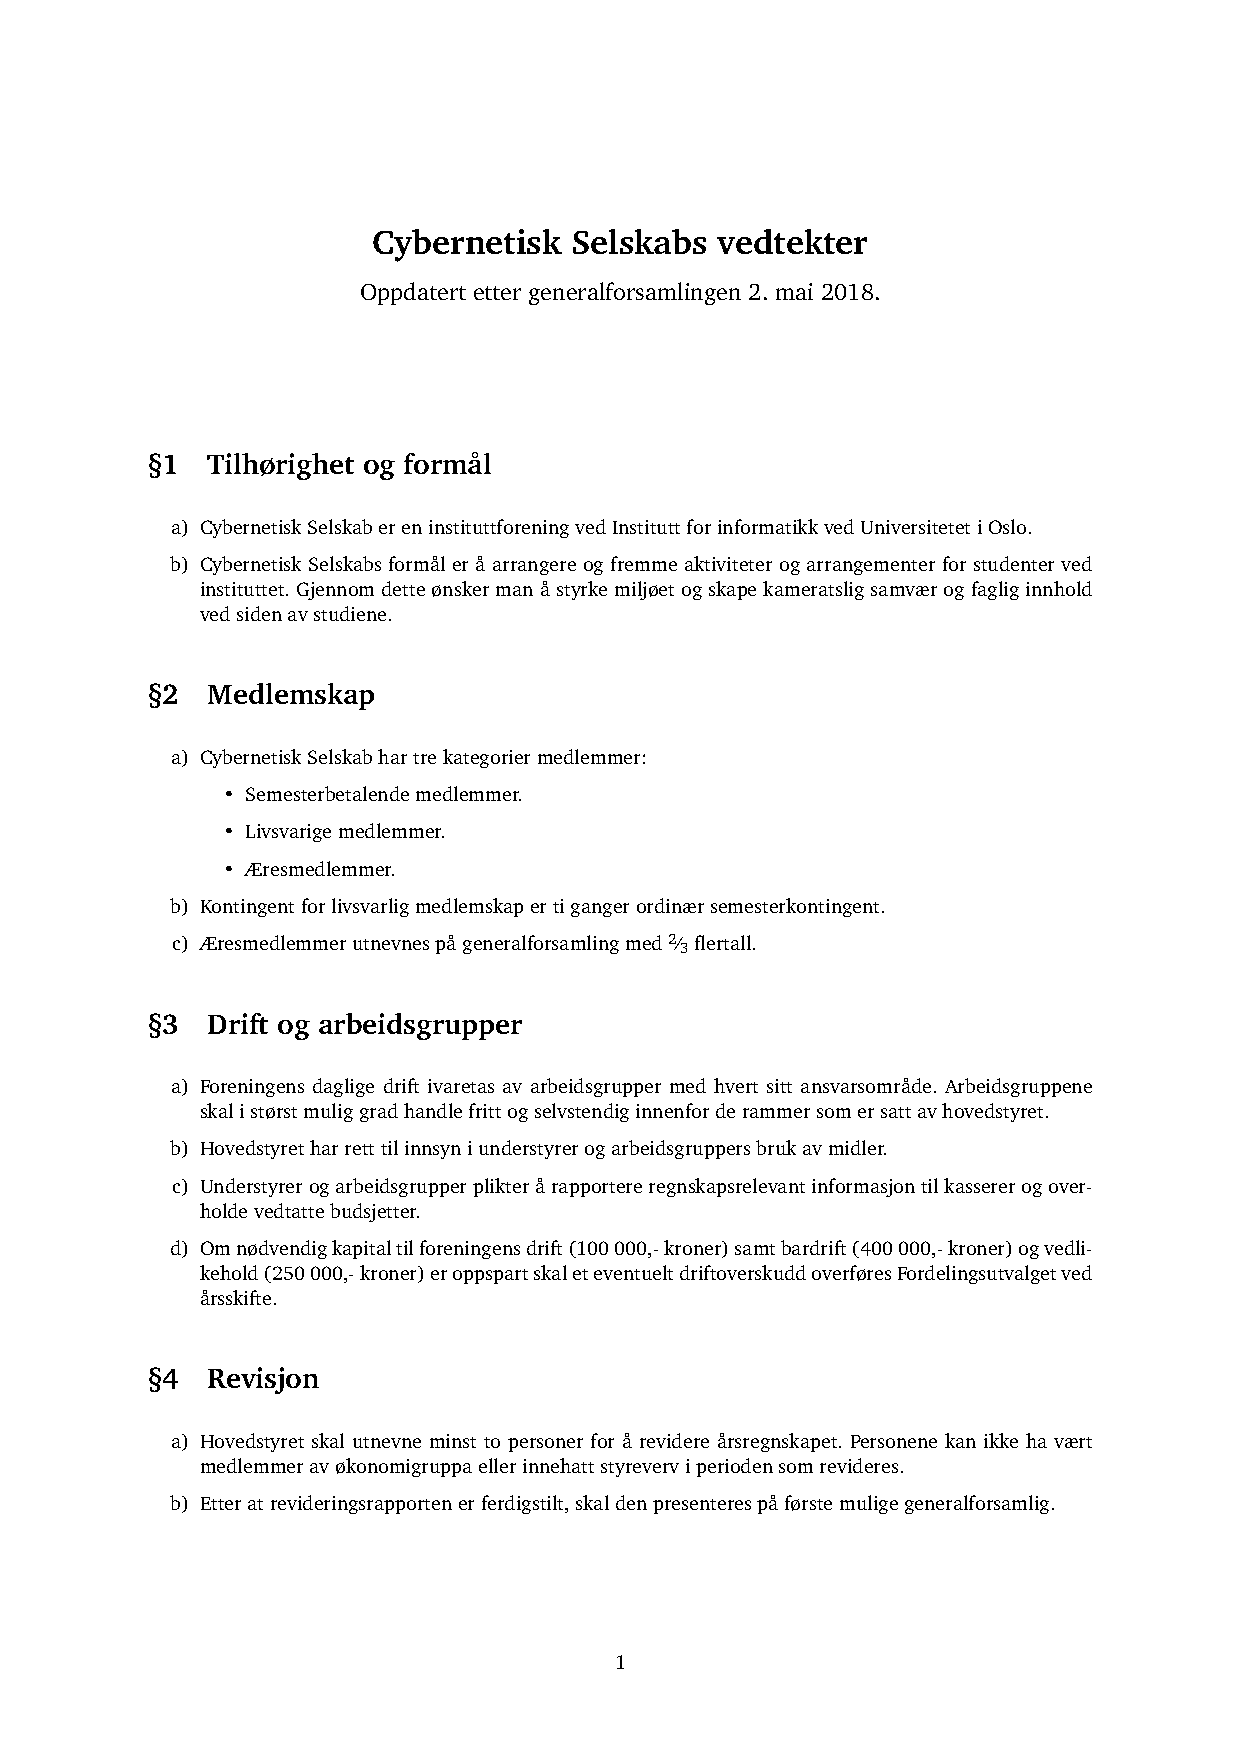
\includepdf[pages=-]{../vedtekter/vedtekter.pdf}

\end{document}
